\documentclass[11pt,openany]{book}
\usepackage{project}
\usepackage{esdiff}
\newcommand{\R}{\mathbb{R}}
\newtheorem{theorem}{Theorem}[section]
\newtheorem{corollary}{Corollary}[theorem]
\newtheorem{lemma}[theorem]{Lemma}
\def\projectauthor{Arav Bhaskaran Jayaprasad\\ (arav.jayaprasad@iiap.res.in)}
\def\projecttitle{Solutions to V.A. Arnold's Mathematical Methods of Classical Mechanics}
\def\projectmonth{\today}
\def\projectdepartment{Theory Department\\ Indian Institute of Astrophysics, Bangalore}
% SECTION STYLE
\setcounter{tocdepth}{2}                            
\setcounter{secnumdepth}{3}
\begin{document}
    \prefrontmatter
    \frontmatter
    \pagenumbering{roman}
    \chapter*{Preface}
These solutions rose out of a personal goal I had set for myself to finish the most mathematically concrete treatment of Classical Mechanics to date, Mathematical Methods of Classical Mechanics by V.A.Arnold. Being a graduate student working on galactic dynamics, I wanted to get a solid foundation on the bread and butter of my field. I was trained in physics without worrying too much about mathematical rigor and this exercise is my attempt at getting acquainted with the tools of differential geometry and its application to Hamiltonian systems. Further, a firm grasp of differential geometry is highly useful when learning general relativity and my goal after finishing Arnold's book is to finally tackle Wald's book on general relativity.\par
Working on galactic dynamics, almost all of the topics in this book are relevant to me except for the section on rigid body dynamics which I have skipped on my first reading. I may or may not get back to this chapter at a later time. Further, given that this is a completely solo effort made worse by my lack of experience with rigorous mathematical proofs, I am in no way claiming that my proofs are correct or as rigorous as they could be and I welcome corrections and suggestions from anyone taking their time to read this document. Working out these proofs as explicitly as possible helped me at least convince myself that a result is right, and as a physicist, this was my primary aim. This work is targeted mainly for physics students as a reference in case they are not accustomed with mathematical proofs and/or don't wish to spend their time trying to work out proofs, but would like to see what they look like.\par
I have tried my best to work things out as explicitly as possible using only the notations and results used in the book. In some sections one has to use results which are presented in further chapters. Since the book has a notoriously bad labeling system for problems, I have written out the problem statement along with the page number where the problem can be found in the book in parenthesis. Questions with self-explanatory answers that are provided in the text are not given different solutions. Notes or ideas that I found useful from different sources during this study are given as footnotes or in boxes where and when relevant. There is also a dedicated subsection proving the theorems of Cartan calculus. 
    \thispagestyle{empty} 
    \tableofcontents \thispagestyle{empty} 
    \mainmatter
    \part{Newtonian Mechanics}
    \chapter{Experimental Facts}
\label{chap0}
\begin{enumerate}
	\item (6) Show that every galilean transformation of the space $ \R\times\R^3$ can be written in a unique way as the composition of a rotation, a translation, and a uniform motion ($ g = g_1 \circ g_2 \circ g_3 $)(thus the dimension of the galilean group is equal to $3+4+3 = 10$).\par
	
	Solution: We first consider a general linear transformation on $ \R\times\R^3$ as the $ 4\times 4 $ matrix $ A $ and an affine transformation $G$ given by $G a = A a+\lambda$ for any $a\in \R\times\R^3$ where $\lambda$ is a constant vector. Since we require $A$ to preserve the galilean structure, $G$ has to preserve the time interval between two events $t(b-a)$, as well as the distance between two simultaneous events $\rho (a, a') = ||a-a'||$. To summarize, $ G $ has to satisfy
	\begin{align}
		t(a-b) &= t(Ga-Gb)\\
		\rho(a,a') &= \rho(Ga, Ga').
	\end{align} 
	We now explicitly write out the transformation of an event $a\in \R\times \R^3$ under $G$.
	\begin{equation}
		Ga = \begin{pmatrix}
			A_{00} & A_{01} & A_{02} & A_{03}\\
			A_{10} & A_{11} & A_{12} & A_{13}\\
			A_{20} & A_{21} & A_{22} & A_{23}\\
			A_{30} & A_{31} & A_{32} & A_{33}
		\end{pmatrix}\begin{pmatrix}
		a^0\\ a^1\\ a^2\\ a^3 
	\end{pmatrix}+\begin{pmatrix}
	\lambda^0\\\lambda^1\\ \lambda^2\\\lambda^3
\end{pmatrix}
		= \begin{pmatrix}
			A_{0i}a^i+\lambda_0\\ A_{1i}a^i+\lambda^1 \\ A_{2i}a^i+\lambda^2\\A_{3i}a^i+\lambda^3
	\end{pmatrix}
	\end{equation}
where repeated indices are summed over $i = 0,..3$. The difference in the coordinate $i = 0$ is taken as the time interval map for $\R \times \R^3$, i.e., $t(a-b) = a^0-b^0$. For the invariance of the time interval between two events $a$ and $b$, we have
\begin{equation}
a^0-b^0 = A_{00}(a^0-b^0) + A_{01}(a^1-b^1)+...
\end{equation}
Since this has to hold for any two events, we are led to the conclusion that $A_{00} = 1$ and $A_{0i} = 0$, $ i = 1,2,3$. Now to preserve distances for two simultaneous events $a$ and $a'$ ($a^0 = a'^0$),
\begin{equation}\label{key}
	\sum_{i,j=1}^3 (A_{ij}(a^j-a'^j))^2 = 	\sum_{i=1}^3 (a^i-a'^i)^2
\end{equation}
Thus the cofactor matrix $A^C = [A^C_{00}]$ obtained by removing the first row and first column must be an orthogonal matrix ($(A^{C})^{\mathrm{T}}A^C = I_3 $, where $I_3$ is the $3\times3$ identity matrix). Thus, a distance and time interval preserving transformation on $\R\times \R^3$ can be written down as 
\begin{equation}\label{genA}
	A = \begin{pmatrix}
		1 & 0 & 0 & 0\\
		v_1&R_{11}& R_{12}& R_{13}\\
		v_2&R_{21}&R_{22} &R_{23} \\
		v_3&R_{31}& R_{31}& R_{33}
		\end{pmatrix}
\end{equation}
where $R_{i,j}$ are the elements of a $3\times 3$ orthogonal matrix $R$, and $v_1, v_2, v_3$ represent the elements $A_{10}, A_{20}, A_{30}$ of $A$ respectively. To see that these terms represent a boost, we consider the action of a transformation $ A_{\mathrm{boost}} $ with $R=I_3$
\begin{equation}\label{key}
	A_{\mathrm{boost}} a = \begin{pmatrix}
			a^0\\
			v_1 a^0 + a^1\\
			v_2 a^0 + a^2\\
			v_3 a^0 + a^3	
		\end{pmatrix}
\end{equation}
which represents the original point moving with a speed given by $\mathbf{v} = (v_1, v_2, v_3)$. Thus, we see that the final galilean transformation can be written down as 
\begin{equation}
	G a  = A_\mathrm{boost}A_\mathrm{orthogonal} a + \lambda
\end{equation}
with \begin{equation}\label{key}
	 A_{\mathrm{boost}} = \begin{pmatrix}
	 	1 & 0 & 0 & 0\\
	 	v_1&1& 0& 0\\
	 	v_2&0&1 &0 \\
	 	v_3&0& 0& 1
	 \end{pmatrix}\hspace{1cm} A_{\mathrm{orthogonal}} = \begin{pmatrix}
	 1 & 0 & 0 & 0\\
	 0&R_{11}& R_{12}& R_{13}\\
	 0&R_{21}&R_{22} &R_{23} \\
	 0&R_{31}& R_{31}& R_{33}
 \end{pmatrix}
\end{equation}
where the boost and rotation operations commute and can be well defined by the combined matrix $A$ from \eqref{genA}.\qed
\item (6) Show that all galilean spaces are isomorphic to each other and, in particular, isomorphic to the coordinate space $\R\times\R^3$.\par
Solution: Let $E, E'$ be galilean spaces with underlying vector space $\R^4$ , i.e., for any $a,b\in E$ or $E'$, $a-b\in \R^4$. If we can find isomorphisms $\phi:E\rightarrow \R\times\R^3$ and $\phi':E'\rightarrow \R\times\R^3$, then we can construct the isomorphism $\phi'^{-1}\circ\phi:E\rightarrow E'$ which is the required isomorphism between two arbitrary galilean spaces.\par
We first construct a map $M:\R^4\rightarrow\R\times\R^3$ that maps the time coordinate to the 0 index (thus the notation $\R\times \R^3$). The time map is a linear map $T:\R^4\rightarrow\R$. Let $e_0,...e_3$ be an arbitrary basis for $\R^4$. Then 
\begin{align}
	v &= v^ie_i\\
	Tv & = v^i (Te_i)
\end{align}
We want to construct a basis $e'_i$ where $T(e'_i) = \delta_{0i}$. Let the required transformation matrix be $M$, $ e'_i = (M^{-1})_i^{j}e_j $. To satisfy the condition, $(M^{-1})_i^{j} T(e_j) = \delta_{0i}\implies T(e_j) = M^i_j\delta_{0i} = M^0_j$. For the remaining indices, we are free to choose any $3\times 4$ matrix such that $M$ is full-rank. Not all $T(e_i)$ can be zero, so assume that at least $T(e_3)$ is non-zero. We set
\begin{equation}\label{key}
	M = \begin{pmatrix}
		T(e_0)&T(e_1)&T(e_2)&T(e_3)	\\
		1 &0 & 0&0\\
		0&1&0&0\\
		0&0&1&0
	\end{pmatrix}.
\end{equation}
 Note that this choice is unimportant as even if all but one of the terms $T(e_i)$ with $i\neq 3$ is zero, we can set the cofactor matrix $[M^C_{0i}]$ to $I_3$ so that $M$ thus defined is full rank. Now,
\begin{align}
	v'^ie'_i &= v^k e_k\\
	v'^i(M^{-1})_i^{j}e_j &= v^k e_k\\
	\implies v'^i (M^{-1})_i^{j} &= v^j\\
	\implies v'^i &= M^i_j v^j
\end{align}
Thus, we have a map $M: \R^4 \rightarrow \R\times\R^3$ such that $Tv = (Mv)^0$ i.e., we have separated the time coordinate $\R$ from the spacial coordinates $\R^3$ of $v$. Since $M$ is full-rank, the map is also invertible. \par
Now let $c\in E$ be fixed. Then we can write any $a\in E$ in the form $a = c + v$ where $v\in \R^4$ (this is effectively choosing an origin), define the map $P_c: E\rightarrow \R^4$ such that $ P_c(a) = a-c = v\in \R^4 $, which is clearly invertible ($P_c^{-1}(v)  = c+v$). Now construct the composite map $\phi_c = M\circ P_c : E\rightarrow\R\times\R^3$. This is the required isomorphism. Note that this is not a canonical isomoprhism as one can make any choice for the "origin" $c\in E$. \qed

\begin{figure}
	\centering
	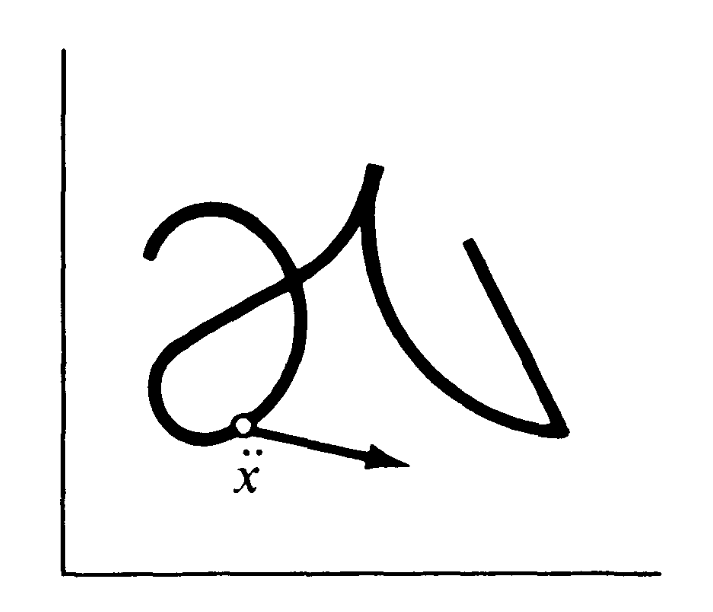
\includegraphics[width=0.5\linewidth]{7}
	\caption[Trajectory of motion of a particle]{}
	\label{fig:7}
\end{figure}

\item (7) Is it possible for the trajectory of a differentiable motion on the plane to have the shape drawn in Figure \ref{fig:7}? Is it possible for the acceleration
vector to have the value shown?\par
Solution: The trajectory shown is a perfectly reasonable motion. However, the acceleration vector shown is not possible. The velocity vector at every point on the curve points in the direction of the tangent to the curve.
The direction of change of the tangent vector is given by the acceleration vector. Clearly, the tangent vector changes "inward" rather than "outward" as indicated by the arrow.
\item (10) Show that if a mechanical system consists of only one point, then
its acceleration in an inertial coordinate system is equal to zero ("Newton's
first law").\par
Solution: If there is only one point  in the system, $\ddot{\mathbf{x}} = \mathbf{f}(t, \mathbf{x},\dot{\mathbf{x}})$ is invariant under translations in time or space and under boosts with constant velocity. This implies \begin{align}\label{key}
	\mathbf{f}(t, \mathbf{x},\dot{\mathbf{x}}) &= \mathbf{f}(t+s, \mathbf{x},\dot{\mathbf{x}})&&\implies  \mathbf{f} = \mathbf{f}(\mathbf{x},\dot{\mathbf{x}}))\\
	\mathbf{f}(\mathbf{x},\dot{\mathbf{x}}))& = 	\mathbf{f}(\mathbf{x}+\mathbf{x_0},\dot{\mathbf{x}}))&&\implies  \mathbf{f} = \mathbf{f}(\dot{\mathbf{x}})\\
	\mathbf{f}(\dot{\mathbf{x}})& = \mathbf{f}(\dot{\mathbf{x}}+\mathbf{v_0}) &&\implies \mathbf{f} = const.
\end{align}
Invariance under orthogonal translations thus implies that $ \mathbf{f} = 0 $.\qed
\item (10) A mechanical system consists of two points. At the initial moment
their velocities (in some inertial coordinate system) are equal to zero. Show
that the points will stay on the line which connected them at the initial
moment.\par
Solution: Let the point be 1 and 2. Choose a coordinate system such that at $t = 0$, $\mathbf{x}_1(0) = a \mathbf{u}_0$, $\mathbf{x}_2(0) = b \mathbf{u}_0$, and $\mathbf{\dot{x}}_1(0) = \mathbf{\dot{x}}_2(0)=0$, where $a$ and $b$ are constants and $u_0$ is a vector parallel to the line joining 1 and 2. The forces on 1 and 2 are given by $\mathbf{f_i}(\mathbf{x_1}-\mathbf{x_2}, \mathbf{\dot{x}}_1-\mathbf{\dot{x}}_2.)$\par
Now, we note that if $\mathbf{v}, \mathbf{w} \in \R^3$ are such that $\mathbf{v} = c \mathbf{w}$ for some $c\in \R$, a rotation $R$ about the $\mathbf{v}$ leaves both vectors unchanged, i.e., $R\mathbf{v} = \mathbf{v}$, $ R\mathbf{w} = \mathbf{w} $ . Then 
\begin{align}
	\mathbf{f}_i(R\mathbf{v},R\mathbf{w}) &= R\mathbf{f}_i(\mathbf{v},\mathbf{w})\\=\mathbf{f}_i(\mathbf{v},\mathbf{w})&\\
	R\mathbf{f}_i(\mathbf{v},\mathbf{w}) = \mathbf{f}_i(\mathbf{v},\mathbf{w})
\end{align}
Thus, if at any point the displacement and relative velocities are parallel to some vector $\mathbf{v}$, the force acting on the particles are also parallel to $\mathbf{v}$.\par
Back to our problem, define the function $F_i(x,y) \mathbf{u_0} \equiv \mathbf{f}_i(x\mathbf{u_0},y\mathbf{u_0})$. Let $y_i(t)$ be the solution to the system $\ddot{y_i} = F_i(y_1-y_2, \dot{y_1}-\dot{y_2})$, with initial conditions $y_1(0) = a$, $y_2(0) = b$, and $\dot{y_1}(0) = \dot{y_2}(0) = 0$. We can show that $\mathbf{x}_i(t) = \mathbf{u_0}y_i(t)$ is a solution to the original problem and thus the points always remain on the line parallel to $u_0$.
\begin{align}
	\ddot{\mathbf{x}}_i& = \mathbf{u_0}\ddot{y}_i\\
	& =\mathbf{u_0} F_i(y_1-y_2, \dot{y_1}-\dot{y_2})\\
	& = \mathbf{f}_i(\mathbf{u_0}(y_1-y_2), \mathbf{u_0}(\dot{y_1}-\dot{y_2})\\
	&=\mathbf{f}_i(\mathbf{x_1}-\mathbf{x_2},\dot{\mathbf{x}}_1-\dot{\mathbf{x}}_2)
\end{align}
This solution is unique since the solution for the $y_i$'s are unique. \qed
\item (10) A mechanical system consists of three points. At the initial moment
their velocities (in some inertial coordinate system) are equal to zero.
Show that the points always remain in the plane which contained them at the
initial moment.\par
Solution: Let the three points be 1, 2, 3. At $t =0$, they lie on some plane $\tau$ with normal $\mathbf{N}$, and we are free to choose inertial coordinates that set the origin as $\mathbf{x}_1(0)$. Then $\mathbf{x}_2(0)-\mathbf{x}_1(0) = \mathbf{u}_0$, $\mathbf{x}_3(0)-\mathbf{x}_1(0) = \mathbf{v}_0$ are vectors that lie on $\tau$ and are perpendicular to $\mathbf{N}$.\par

We now note that reflections are also distance preserving transformations and are also a valid galiliean transformations\footnote{Reflections are discrete transformations as opposed to the continuous translation, boost and rotation. The set of all galilean transformations barring rotations forms a Lie Group (see \ref{chap8}).} (this is a problem in this chapter which we will argue now to proceed with this problem). Reflections are orthogonal transformations with $\mathrm{det}G = -1$. Invariance  with respect to reflections means that there are no preferred orientations of coordinates in space. Thus we have the relation 
\begin{equation}
	\mathbf{F}(G\mathbf{x},G\dot{\mathbf{x}}) = G \mathbf{F}(\mathbf{x},\dot{\mathbf{x}})
\end{equation}

The forces that enter the equations of motion are functions of $\mathbf{x_i}-\mathbf{x_j}$ and $\dot{\mathbf{x_i}}-\dot{\mathbf{x_j}}$ , i.e., $ \mathbf{f}_i  = \mathbf{f}_i(\mathbf{x_2}-\mathbf{x_1},\mathbf{x_3}-\mathbf{x_1},\dot{\mathbf{x_2}}-\dot{\mathbf{x_1}},\dot{\mathbf{x_3}}-\dot{\mathbf{x_1}})$. Let $\mathbf{w_1}, \mathbf{w_2}, \mathbf{w_3}, \mathbf{w_4}\in \textit{Span}(\mathbf{u_0}, \mathbf{v}_0)$, and G denote the reflection through the direction $\mathbf{N}$. Clearly, $G\mathbf{u}_0 = \mathbf{u}_0$ and $G\mathbf{v}_0 = \mathbf{v}_0$ and thus similar relations hold for the $\mathbf{w}_i$. Let $\mathbf{f}_i(\mathbf{w_1}, \mathbf{w_2}, \mathbf{w_3}, \mathbf{w_4}) = \mathbf{f}_{i}^{||}+ \mathbf{f}_{i}^{\perp}$ denote the components parallel and perpendicular to the plane $\tau$ (or perpendicular and parallel the normal $\mathbf{N}$) respectively. Now
\begin{equation}\label{incons1}
	G \mathbf{f}_i = G\mathbf{f}_{i}^{||} + G \mathbf{f}_{i}^{\perp} = \mathbf{f}_{i}^{||} -  \mathbf{f}_{i}^{\perp}.
\end{equation}
But from galilean invariance we have
\begin{equation}\label{incons2}
	G \mathbf{f}_i(\mathbf{w}_1,...) = \mathbf{f}_i(G\mathbf{w}_1,...) = \mathbf{f}_i(\mathbf{w}_1,...) = \mathbf{f}_{i}^{||}+ \mathbf{f}_{i}^{\perp}
\end{equation}
Equations \eqref{incons1} and \eqref{incons2} imply that $ \mathbf{f}_{i}^{\perp} = 0$. Thus if all arguments $\mathbf{w}_i$ lie on a plane, the forces $\mathbf{f}_i$ on all the particles also lies on the same plane.  \par

Now we define \begin{multline}\label{key}
	\mathbf{f}_i(a_1\mathbf{u_0}+b_1\mathbf{v_0}, ...,a_4\mathbf{u_0}+b_4\mathbf{v_0})\equiv\\ \mathbf{u_0}F_i^0(a_1, b_1,...a_4,b_4)+\mathbf{v_0}F_i^1(a_1,b_1,...,a_4,b_4)
\end{multline}
Let $y_i^j(t)$ be the solutions for $\ddot{y}_i^j = F_i^j(y_2^j-y_1^j, y_3^j-y_1^j ,\dot{y}_2^j -\dot{y}_1^j, \dot{y}_3^j-\dot{y}_2^j)$, with initial conditions $y_1^0(0) = y_1^1(0) = 0$, $y_2^0(0) = 1, y_2^1(0) = 0$, $y_3^0(0) = 0, y_3^1(0) = 1$ and $\dot{y}_i^j(0) = 0$ for $i = 1,2,3$ and $j = 1,2$.  Consider solutions of the form $ 	\mathbf{x}_i(t) = y_i^0(t) \mathbf{u}_0 + y_i^1(t) \mathbf{v}_0 $. Similar to the previous problem, it can be shown that these are also valid solutions. Now the system of differential equations for the $y_i^j$ are 6 second order equations with 12 initial conditions and thus possess a unique solution and thus, this solution for the $\mathbf{x}_i$ are unique. Thus we have shown that the trajectories of three particles stay on a plane if they started from rest in some inertial coordinate.\qed
\item (10) A mechanical system consists of two points. Show that for any
initial conditions there exists an inertial coordinate system in which the
two points remain in a fixed plane.\par
Solution: Let the two points be 1 and 2. They have initial conditions $\mathbf{x}_1(0) = \mathbf{a}_1$, $\mathbf{x}_2(0) = \mathbf{a}_2$, $\dot{\mathbf{x}}_1(0) = \mathbf{u}_0$, and $\dot{\mathbf{x}}_2(0) = \mathbf{v}_0$. The equations of motion take the form\begin{equation}\label{key}
	\ddot{\mathbf{x}}_i = \mathbf{f}_i(\mathbf{x}_1-\mathbf{x}_2, \dot{\mathbf{x}}_1-\dot{\mathbf{x}}_2)
\end{equation}
Let $\mathbf{r}= \mathbf{x}_1-\mathbf{x}_2$ and $\mathbf{v} = \dot{\mathbf{x}}_1-\dot{\mathbf{x}}_2)$. Consider the vector $\mathbf{L} = \mathbf{r}\times\mathbf{v}$. If the direction of $\mathbf{L}$ does not change with time, $\mathbf{r}$ and $\mathbf{v}$ lie on a plane perpendicular to $\mathbf{L}$ that moves at some speed parallel to $\mathbf{L}$. Now,\begin{align}\label{key}
	\dot{\mathbf{L}}& = \dot{\mathbf{r}}\times\mathbf{v}+\mathbf{r}\times\dot{\mathbf{v}}\\
&=	\mathbf{r}\times\ddot{\mathbf{r}}
\end{align}
At some instant, let $ G $ denote reflection about the plane on which the particles lie that is perpendicular to $\mathbf{L}$. Using the invariance of $\mathbf{r}$ and $\mathbf{v}$ on this reflection, we get $G \ddot{\mathbf{r}} = G\mathbf{f}_1(\mathbf{r},\mathbf{v})-G\mathbf{f}_2(\mathbf{r},\mathbf{v}) =\mathbf{f}_1(G\mathbf{r},G\mathbf{v})-\mathbf{f}_2(G\mathbf{r},G\mathbf{v}) = \mathbf{f}_1(\mathbf{r},\mathbf{v})-G\mathbf{f}_2(\mathbf{r},\mathbf{v}) = \ddot{\mathbf{r}} $. Thus, we have shown that at every instant of the motion, the relative acceleration $\ddot{\mathbf{r}}$ is perpendicular to $\mathbf{L}$ and thus coplanar with $\mathbf{r}$ and $\mathbf{v}$. Thus the direction of $\mathbf{r}\times\ddot{\mathbf{r}}$ is parallel to that of $\mathbf{L}$ and the direction of $\mathbf{L}$ does not change with time. Further, one can also show that $G \ddot{\mathbf{x}}_i =G\mathbf{f}_i(\mathbf{r},\mathbf{v}) = \mathbf{f}_i(G\mathbf{r},G\mathbf{v}) = \mathbf{f}_i(\mathbf{r},\mathbf{v}) = \mathbf{x}_i$ and thus the acceleration of the particles also lies on the plane perpendicular to $\mathbf{L}$ at every instant.\par
We now find the inertial coordinates in which the particles appears to move on a plane. At every instant of motion, the component of the velocity of 1 parallel to $\mathbf{L}$ is given by 
\begin{equation}\label{key}
	\dot{\mathbf{x}}_1^{||} = \dot{\mathbf{x}}_1.\frac{(\mathbf{r}\times\mathbf{v})}{|(\mathbf{r}\times\mathbf{v}|} = -\dot{\mathbf{x}}_1.\frac{(\mathbf{r}\times\dot{\mathbf{x}}_2)}{|(\mathbf{r}\times\mathbf{v}|} = \mathbf{r}.\frac{(\dot{\mathbf{x}}_1\times\dot{\mathbf{x}}_2)}{|(\mathbf{r}\times\mathbf{v}|}
\end{equation}
where we have used the properties of the triple product. Similarly,
\begin{equation}\label{key}
	\dot{\mathbf{x}}_2^{||} = \dot{\mathbf{x}}_2.\frac{(\mathbf{r}\times\mathbf{v})}{|(\mathbf{r}\times\mathbf{v}|} = \dot{\mathbf{x}}_2.\frac{(\mathbf{r}\times\dot{\mathbf{x}}_1)}{|(\mathbf{r}\times\mathbf{v}|} = \mathbf{r}.\frac{(\dot{\mathbf{x}}_1\times\dot{\mathbf{x}}_2)}{|(\mathbf{r}\times\mathbf{v}|} = \dot{\mathbf{x}}_1^{||}
\end{equation}
Now, we have shown that at every instant of the motion, $\ddot{\mathbf{x}}_i$ is perpendicular to $\mathbf{L}$. This the components of the velocity parallel to $\mathbf{L}$ are constant and are set by the initial conditions. We define $\mathbf{v}_\mathrm{inertial} \equiv \dot{\mathbf{x}}_1^{||} = \dot{\mathbf{x}}_2^{||}$ given by \begin{equation}\label{key}
\mathbf{v}_\mathrm{inertial} = 	(\mathbf{a}_1-\mathbf{a}_2).\frac{(\mathbf{u}_0\times\mathbf{v}_0)}{|\mathbf{u}_0\times\mathbf{v}_0|}
\end{equation}
Thus, by carrying out a boost with velocity $ \mathbf{v}_\mathrm{inertial} $, the velocities of the particles parallel to $\mathbf{L}$ vanish and one sees the particles moving on a plane perpendicular to $\mathbf{L}$.\qed
\item (11) Show that mechanics "through the looking glass" is identical
to ours.\par
Solution: As we have mentioned before, reflections are orthogonal transformations and thus are distance preserving maps. They also form a subset of galilean transformations. If a motion $\mathbf{x}_i(t)$ satisfies $\ddot{\mathbf{x}}_i = \mathbf{F}_i(\mathbf{x},\dot{\mathbf{x}})$, then so does $G\mathbf{x}_i(t)$ and thus 
\begin{equation}
	G\ddot{\mathbf{x}} = G \mathbf{F}(\mathbf{x},\dot{\mathbf{x}})=\mathbf{F}(G\mathbf{x},G\dot{\mathbf{x}})
\end{equation}
\item(11) Is the class of inertial systems unique?\par
Solution: Given in text.
	\end{enumerate}


    \chapter{Investigations of the Equations of Motion}\label{chap2}

\begin{enumerate}
	\item (16) Show that through every phase point there is one and only one	phase curve.\par 
	Solution: The phase flow is given by the equations
	\begin{equation}\label{flow}
		\dot{x} = y\hspace{1cm} \dot{y} = f(x).
	\end{equation}
	The equation for $y$ can be written as
	\begin{align}
		\diff{y}{x} y &= f(x)\\
		\implies \int_{y_0}^{y} y'\mathrm{d}y' & = \int_{x_0}^x f(x')\mathrm{d}x\\
		\implies \frac{y^2}{2} - F(x) &= \frac{y_0^2}{2} - F(x_0) = const.\label{eqflow}
	\end{align}
where $(x_0,y_0)$ are initial conditions, and $F(x)$ is the anti-derivative of $f(x)$, which is defined up to a constant. We note that due to the appearance of $F$ on both sides of equation \eqref{eqflow}, the choice of this arbitrary constant is not important. The equation \eqref{eqflow} is the equation of a 1-D curve in phase space that passes through the point $(x_0,y_0)$. This is a well defined unique curve that is determined by only the initial conditions, which can be taken at any point on the curve. \qed
\item (18) Prove this (that the local maximum points ofthe
potential energy are unstable, but the minimum points are stable equilibrium
positions).\par
Problem: The solution to this is straightforward. $f(x) = -\mathrm{d}U/\mathrm{d}x = U'(x)$, where $U$ is the potential. If $x_0$ is an equilibrium point, $U'(x_0) = 0$. Thus the force at a point $x_0+\epsilon$ is given by\begin{equation}\label{key}
	f(x_0+\epsilon) = -\epsilon U''(x_0) + \mathcal{O}(\epsilon^2).
\end{equation}
If the point $x_0$ is a minimum, $U''(x_0)>0$ and thus the force tends to drive the body back to equilibrium (stable). On the other hand, if it is a maximum, $U''(x_0)<0$ and the force tends to drive the body away from equilibrium(unstable).
\item (18) How many phase curves make up the separatrix (figure eight) curve, corresponding to the level $E_2$ ?\par
Solution: Three: two 1-D curves, and a single unstable equilibrium point.
\item(18) Determine the duration of motion along the separatrix.\par
Solution: As the particle approaches the  equilibrium point, it's velocity starts to tend towards zero from energy conservation, while the force acting on it also tends to 0. To estimate the time, we use the result from the next problem which we will prove soon.
\begin{equation}\label{key}
	\Delta t = \int_{x_1}^{x_2}\frac{\mathrm{d}x}{\sqrt{2(E-U(x))}}
\end{equation}
Let $E = U(x_0)$, $x_1 = x_0-\epsilon_0$, and $x_2 = x_0$. We can change the integration variable to $\epsilon$ and expanding the potential about $x_0$, we have $U(x_0-\epsilon) =  U(x_0) + U''(x_0)\epsilon^2/2$. Thus, to leading order in $\epsilon$ we get
\begin{equation}\label{key}
	\Delta t \sim \int_{\epsilon_0}^{0}\frac{\mathrm{d}\epsilon}{\sqrt{-U''(x_0)\epsilon^2}}
\end{equation}
which clearly diverges logarithmically. The term under the square root is positive as $U''(x_0)<0$ due to $x_0$ being a maxima. Thus the time taken is infinite.\par
Alternatively as mentioned by Arnold, there is a unique phase curve (the 0 dimensional equilibrium point) at the phase point $(x_0, 0)$. Using the fact that there is only once phase curve passing through every point, we conclude that seperatrix trajectory always moves towards the equilibrium point but never reaches it and thus takes infinite time.

\item \label{timeprob}(18) Show that the time it takes to go from $x_1$ to $x_2$ (in one direction)is equal to
\begin{equation}\label{key}
	t_2 -t_1 = \int_{x_1}^{x_2}\frac{\mathrm{d}x}{\sqrt{2(E-U(x))}}
\end{equation}
Solution: \begin{align}
	E &= T+ U = \dot{x}^2/2+U(x)\\
	\implies \dot{x}^2& = 2(E- U(x))\\
	\implies \int_{t_1}^{t_2}\mathrm{d} t & = \int_{x_1}^{x_2}\frac{\mathrm{d}x}{\sqrt{2(E-U(x))}}
\end{align}\qed

\item (19) Draw the phase curves, given the potential energy graph in Figure 11 (of Arnold's Book).
Solution: Given in text
\item (19) Draw the phase curves for the "equation of an ideal planar pendulum": $\ddot{x} = -\sin x$.\par
Solution: The procedure for drawing these images is to plot the potential and work out the turning points corresponding to a given energy. The plot generated using the StreamPlot function in Mathematica is shown in figure \ref{fig:2pendulumstream}
% TODO: \usepackage{graphicx} required
\begin{figure}
	\centering
	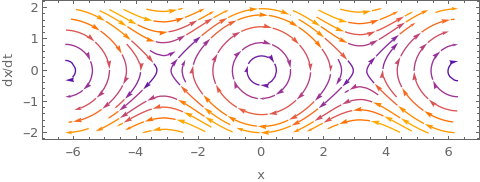
\includegraphics[width=0.7\linewidth]{2_pendulumstream}
	\caption{Phase curves of planar pendulum}
	\label{fig:2pendulumstream}
\end{figure}

\item (19) Draw the phase curves for the "equation of a pendulum on a rotating axis": $\ddot{x} = -\sin x + M$
Solution: See figure \ref{fig:2pendulumstreamrot}.
\begin{figure}
	\centering
	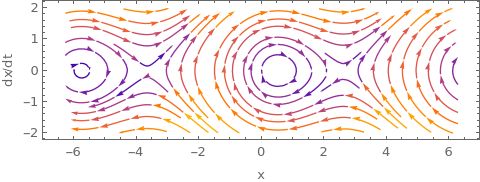
\includegraphics[width=0.7\linewidth]{2_pendulumstreamrot}
	\caption{Phase curves of rotating pendulum}
	\label{fig:2pendulumstreamrot}
\end{figure}
\item (19) Find the tangent lines to the branches of the critical level corresponding to maximal potential energy $E = U(\xi)$ (Figure \ref{fig:2critical}).\par
% TODO: \usepackage{graphicx} required
\begin{figure}
	\centering
	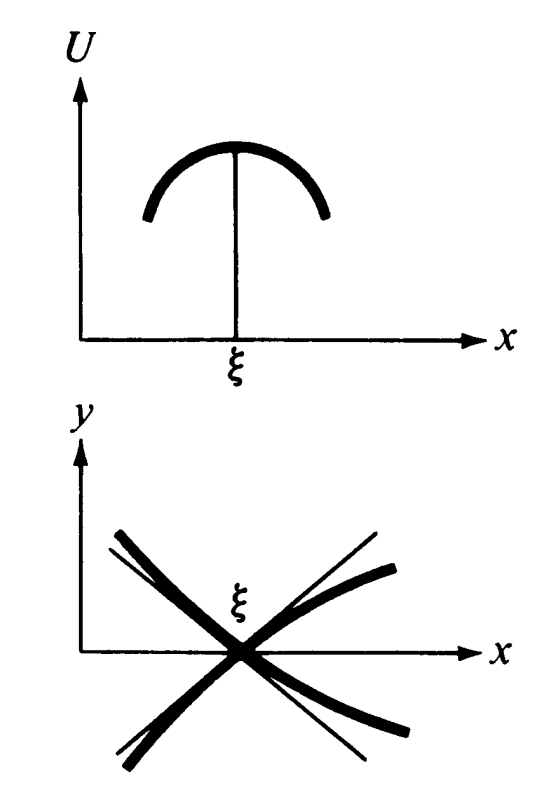
\includegraphics[width=0.5\linewidth]{2_critical}
	\caption{Critical energy level lines}
	\label{fig:2critical}
\end{figure}
Solution:  From the first problem in this chapter, we have \begin{equation}\label{key}
		\frac{y^2}{2} +U(x) = \frac{y_0^2}{2} + U(\xi) = U(\xi)\implies y = \pm\sqrt{2(U(\xi)-U(x))}
\end{equation}
Expanding $U(x)$ near the equilibrium point $\xi$, $U(x) = U(\xi)+(x-\xi)U'(\xi) +(x-\xi)^2 U''(\xi)/2 +\mathcal{O}((x-\xi)^3)$, which finally gives
\begin{equation}
	y = \pm (x-\xi)\sqrt{U''(\xi)}
\end{equation}
\item (20) Let $S(E)$ be the area enclosed by the closed phase curve corresponding to the energy level $E$. Show that the period of motion along this curve is equal to $T = \mathrm{d}S/\mathrm{d}E$.\par

Solution: Let the motion have turning points $x_1, x_2$ i.e., $U(x_1) = U(x_2) = E$, with $x_1<x_2$. Then the area under the phase space curve is given by \begin{align}\label{area}
	S(E) &= \int_{x_1}^{x_2}\mathrm{d}x|\dot{x}|+\int_{x_2}^{x_1}\mathrm{d}x(-|\dot{x}|)\\
	& = 2\int_{x_1}^{x_2}\mathrm{d}x \sqrt{2(E-U(x))}
\end{align}
where the first and second terms in equation \eqref{area} represent the motion from $x_1$ to $x_2$ and the reverse motion with negative velocity from $x_2$ to $x_1$ respectively. Now
\begin{align}
	\frac{\mathrm{d}S}{\mathrm{d}E} &= 2\int_{x_1}^{x_2}\frac{\mathrm{d}x}{\sqrt{2(E-U(x))}}\\
	&= T_{x_1\rightarrow x_2} + T_{x_2 \rightarrow x_1}
\end{align}
which gives the total time period of the motion. We have used the result of problem \ref{timeprob}.\qed
\item (20) Let $E_0$ be the value of the potential function at a minimum point $\xi$. Find the period $T_0$ of small oscillations in a neighborhood of the point $\xi$, where $T_0$ = $\lim_{E\rightarrow E_0} T(E)$.\par
Solution: Taylor expand the potential $U(x)$ near the minimum point
\begin{equation}\label{key}
	U(x) = E_0 + \frac{(x-\xi)^2}{2} U''(\xi) + \mathcal{O}((x-\xi)^3)
\end{equation}
The equation of motion gives
\begin{equation}\label{eom}
	\ddot{x} = -U'(x) = -(x-\xi)U''(\xi).
\end{equation}
Let $z = x-\xi$. Equation \eqref{eom} can be written as $\ddot{z} = -z U''(\xi)$. This is the equation of a 1-D harmonic oscillator with frequency $\omega = \sqrt{U''(\xi)}$. Thus the time period of the motion is given by $T_0 = 2\pi/\sqrt{U''(\xi)}$
\item (20) Consider a periodic motion along the closed phase curve corresponding to the energy level $E$. Is it stable in the sense of Liapunov?\par
Solution: An equilibrium point $\xi$ is said to be Liapunov stable if $\forall \epsilon>0, \exists$ $\delta(\epsilon)>0$ such that if $|x(0)-\xi|<\delta(\epsilon)$ then $|x(t)-\xi|<\epsilon$ $\forall t>0$. Simply put, we must be able to confine the motion to an arbitrarily small region of configuration space around $\xi$ by starting the motion sufficiently close to $\xi$. However, for a given periodic motion with turning points $x_1<\xi<x_2$, this is not possible for any $\epsilon<\min(\xi-x_1, x_2-\xi)$, as $|x(t)-\xi|$ will exceed this value at some point of the periodic orbit. Thus the motion is not Liapunov stable.
\item (21) Show that the system with potential energy $U = - x^4$ does not define a phase flow.\par
Solution: In order for the motion in a potential to constitute a phase flow, it must be possible to extend the solution to the entire time axis. If the motion reaches infinity in a finite amount of time, then the group properties given in the text are destroyed and thus the the motion will not define a phase flow. We now calculate the time period of motion to infinity in this potential. \par
There are two cases: $E>0$ and $E<0$. For $E<0$, let the particle have initial condition $x(0) = x_0$, $\dot{x}(0) = 0$. Its energy is given by $E = U(x_0)$. The time period for motion up to a point $x_1$ is given by (\ref{timeprob})\begin{align}\label{key}
	T &= \int_{x_0}^{x_1}\frac{\mathrm{d}x}{\sqrt{2(E-U(x))}}\\
	&\int_{x_0}^{x_1}\frac{\mathrm{d}x}{\sqrt{2(x^4-x_0^4)}}\\
\end{align}
Let $y^4 = x^4/x_0^4>0$  and let $x_1\rightarrow\infty$. Then 
\begin{equation}
	T_{\infty} = \frac{1}{\sqrt{2}x_0}\int_{1}^\infty\frac{\mathrm{d}y}{\sqrt{y^4-1}} = \frac{1}{2x_0} K\bigg(\frac{1}{\sqrt{2}}\bigg)\sim \frac{1.043}{x_0} ,
\end{equation}
where $K$ is the complete elliptic integral of the first kind (see Gradshteyn and Ryzhik - Table of Integrals, Series, and Products 7th ed.(GR) 3.166-17). For $E>0$, let $x(0) = x_0$, $\dot{x}(0) = v_0$. Its energy is given by $E = m v_0^2/2 + U(x_0)$\begin{equation}\label{key}
	T = \int_{x_0}^{x_1}\frac{\mathrm{d}x}{\sqrt{2(mv_0^2/2+x^4-x_0^4)}}.
\end{equation}
Let $z^4 = x^4/(mv_0^2/2-x_0^4)>0$ and let $x_1\rightarrow\infty$. Then 
\begin{equation}
	T_{\infty} = \frac{1}{\sqrt{2(mv_0^2/2-x_0^4)}}\int_{z_0}^\infty\frac{\mathrm{d}z}{\sqrt{z^4+1}} = \frac{1}{\sqrt{2(mv_0^2/2-x_0^4)}} F\bigg(\alpha, \frac{1}{\sqrt{2}}\bigg),
\end{equation}
where $z_0 = x_0^4/(mv_0^2/2-x_0^4)$, $F$ is the incomplete elliptic integral of first kind (GR-3.166-1) and $\alpha = (z_0^2-1)/(z_0^2+1)$.
Thus, we see that in the quartic potential, the particle reaches infinity at a finite time, and thus one cannot define a one-parameter group of diffeomorphisms. \qed
\item Show that if the potential energy is positive, then there is a phase flow.\par
Solution: Let $U(x)>0$. For bound orbits, the motion is periodic and thus can be extended to the entire time axis. For unbound orbits, let at $t=0$, $x(0) = x_0$, $\dot{x}(0)= 0$, so that the energy $E = U(x_0)>0$. The time to reach some $x_1$ is given by
\begin{equation}
	T = \int_{x_0}^{x_1}\frac{\mathrm{d}x}{\sqrt{2(U(x_0)-U(x))}}>\int_{x_0}^{x_1}\frac{\mathrm{d}x}{\sqrt{2U(x_0)}} = \frac{x_1-x_0}{\sqrt{2U(x_0)}}
\end{equation}
where we have used the fact that $U$ is positive and the orbit is unbound. Thus we see that the time period is bounded below by a linear function of $x$, and thus, for ever finite $t$, the motion in $x$ is finite, and thus the motion can be extended to the whole time axis. Thus we can define a phase flow. 
\item  Draw the image of the circ1e $x^2 + (y - 1)^2 < 1/4$ under the action of the transformation of the phase flow for the equations (a) of the "inverse pendulum," $\ddot{x} = x$ and (b) of the "nonlinear pendulum," $\ddot{x} = -\sin x$.\par
Solution: The stable equilibrium points and seperatrix can easily be inferred by observing the potential. We will derive the general solutions for the trajectories here, which can be plotted using any graphing software (DESMOS, Mathematica, etc).\par
\begin{enumerate}
	\item The general solution to the ODE can be seen to be 
\begin{align}\label{key}
	x(t) &= a e^t + b e^{-t}\\
	y(t) &= a e^t - b e^{-t}.
\end{align}
Using initial conditions $y(0) = y_0$, $x(0) = x_0$, we get
\begin{align}\label{key}
	x(t) &=\frac{x_0+y_0}{2}e^t + \frac{x_0-y_0}{2} e^{-t}\\
	y(t) &= \frac{x_0+y_0}{2} e^t - \frac{x_0-y_0}{2} e^{-t}.
\end{align}
This can be inverted easily by using $(x,y)$ as the initial conditions and evolving the system to $-t$. This gives
\begin{align}\label{key}
	x_0 &=\frac{x+y}{2}e^{-t} + \frac{x-y}{2} e^{t}\\
	y_0 &= \frac{x+y}{2} e^{-t} - \frac{x-y}{2} e^{t}.
\end{align}
One can now plot the region in the $(x,y)$ plane at time $t$ corresponding to $(x_0,y_0)$ lying in the original circle at $t=0$. They are ellipses as seen in figure \ref{invp}.
\begin{figure}[!h]
	\centering
	\subfigure[$t = 0$]{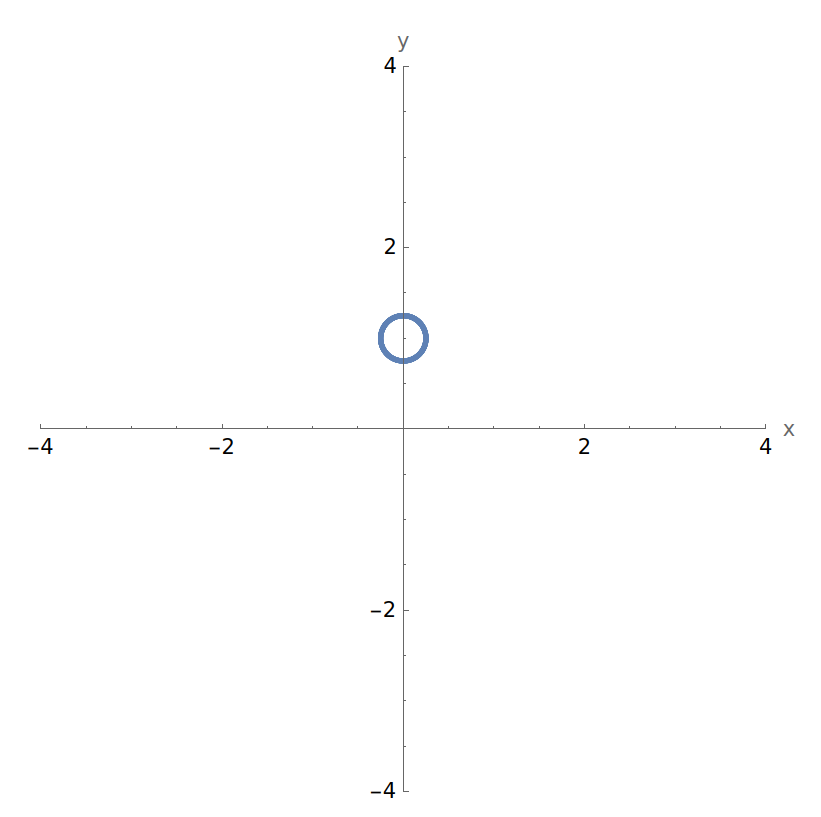
\includegraphics[width=.3\textwidth]{2_invpendulum}}
	\subfigure[$t = 0.3$]{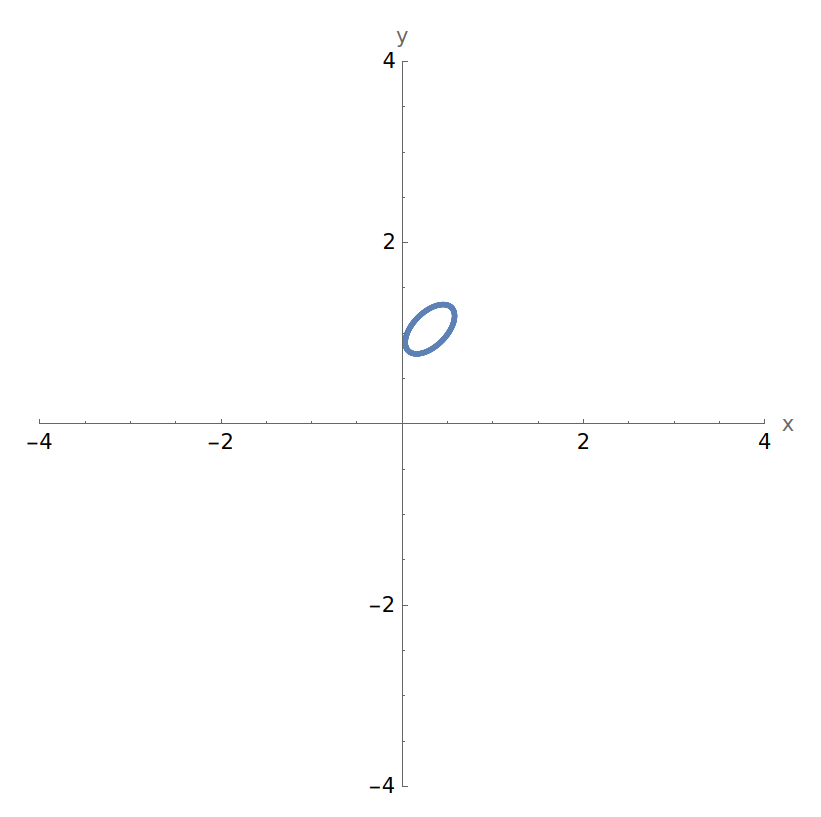
\includegraphics[width=.3\textwidth]{2_invpendulum1}}
	\subfigure[$t = 1$]{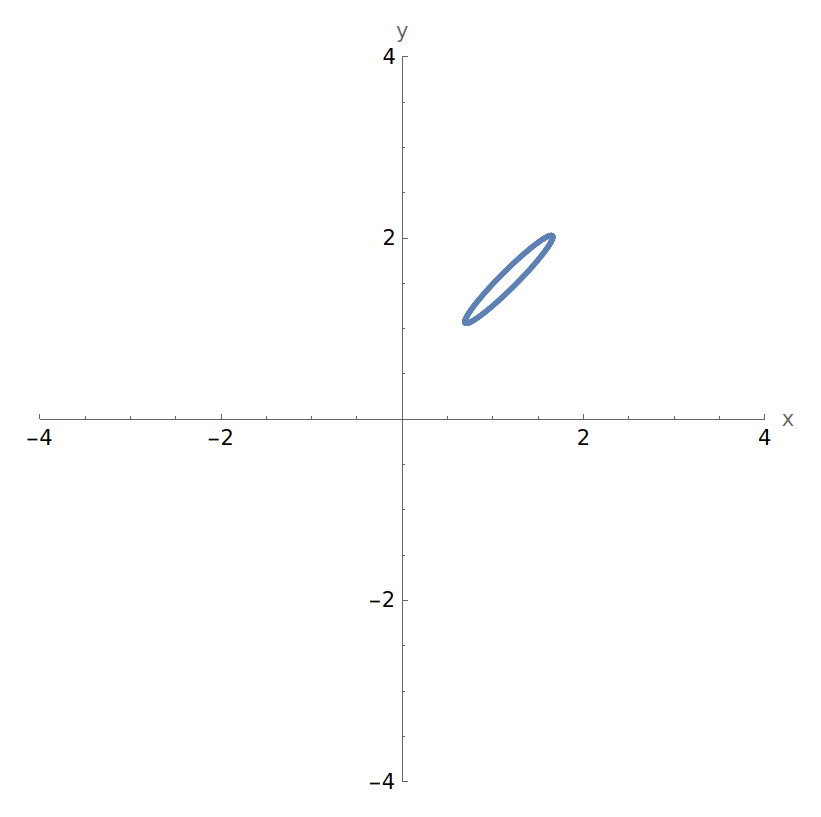
\includegraphics[width=.3\textwidth]{2_invpendulum2}}
	
	\caption{Phase plot for the inverse pendulum. The points lying on the boundary of the initial circle and subsequent motion are shown in blue.}
	\label{invp}
\end{figure}
\item This system is a lot more involved and uses elliptic integrals. The results and definitions used here may be found in GR-8.1. The ODE for $x$ can be written as 
\begin{align}
	y\mathrm{d}y & = -\sin x \mathrm{d}x\\
	y^2-y_0^2 &= 2(\cos x-\cos x_0)\label{yeqnl}\\
	y & = \sqrt{y_0^2 + 4(\sin ^2 (x_0/2)-\sin ^2 (x/2))}\\
	\mathrm{d}t & = \frac{\mathrm{d}x}{\sqrt{y_0^2 + 4(\sin ^2 (x_0/2)-\sin ^2 (x/2))}}\\
	t& = \int_{x_0}^{x}\frac{\mathrm{d}x}{2\sqrt{k_0^2-\sin^2(x/2)}},
\end{align}
where we have used standard trigonometric formulae and defined $k_0^2 \equiv y_0^2/4 + \sin^2(x_0/2)$. Define the variable $z$ such that $\sin z = \sin(x/2)/k_0$. Carrying out the change of variables, it is easy to see that
\begin{align}
	t & = \int_{z_0}^{z}\frac{\mathrm{d}z}{\sqrt{1-k_0^2\sin^2(z)}}\\
	&= F(z,k_0) - F(z_0,k_0),
\end{align}
where $ \sin z_0 = \sin(x_0/2)/k $. To invert this equation, we use the definition of the Jacobi elliptical integrals (see GR-8.14)\begin{align}\label{key}
	u &\equiv \int_0^{\mathrm{am} (u,k)}\frac{\mathrm{d}\alpha}{1-k^2\sin^2\alpha}\\
	&\equiv \int_0^{\mathrm{sn}(u,k)}\frac{\mathrm{d}t}{\sqrt{(1-t^2)(1-k^2t^2)}}
\end{align}
We thus get,\begin{align}\label{key}
	z &= \mathrm{am}(t + F(z_0,k_0),k_0)\\
	\sin z & = 	\mathrm{sn}(t + F(z_0,k_0),k_0)\\
	x(t)& = 2\arcsin(k_0 \cdot \mathrm{sn}(t + F(z_0,k_0),k_0)).
\end{align}
Now, using equation \eqref{yeqnl}, we get
\begin{align}
	y(t) &= 2\sqrt{k_0^2 - k_0^2 \mathrm{sn}^2(t + F(z_0,k_0),k_0)}\\
	& = 2 k_0 \cdot\mathrm{cn}(t + F(z_0,k_0),k_0).
\end{align}
Similar to the previous part, one can obtain the initial conditions $(x_0,y_0)$ as a function of $(x(t),y(t))$
\begin{align}
	x_0 &= 2\arcsin(k\cdot\mathrm{sn}(-t+F(z,k),k))\\
	y_0 &= 2k\cdot\mathrm{cn}(-t + F(z,k),k).
\end{align}
The circle condition may now be enforced on the initial condition which then leads to a constraint on the coordinates at later times. Qualitatively, all points trace an elliptical trajectory, with the point starting from $(0,3/4)$ having the smallest size and the point starting from $(5/4,0)$ being the largest, and all other points lying in-between. There is unstable equilibrium at $x = \pm \pi$ and a stable equilibrium at $x=0$. Any point with energy higher than the maximum value of the potential, 1, is unbound. At $x = 0$, points starting with $y>2$ are unbound. The curves starting from $y =\pm2$ and $x = 0$ form the seperatrix. As the motion proceeds, the circle is smeared more and more in phase space (phase mixing). The phase plot is shown in figure \ref{FIGURE LABEL}.
\begin{figure}[!h]
	\centering
	\subfigure[$t = 0$]{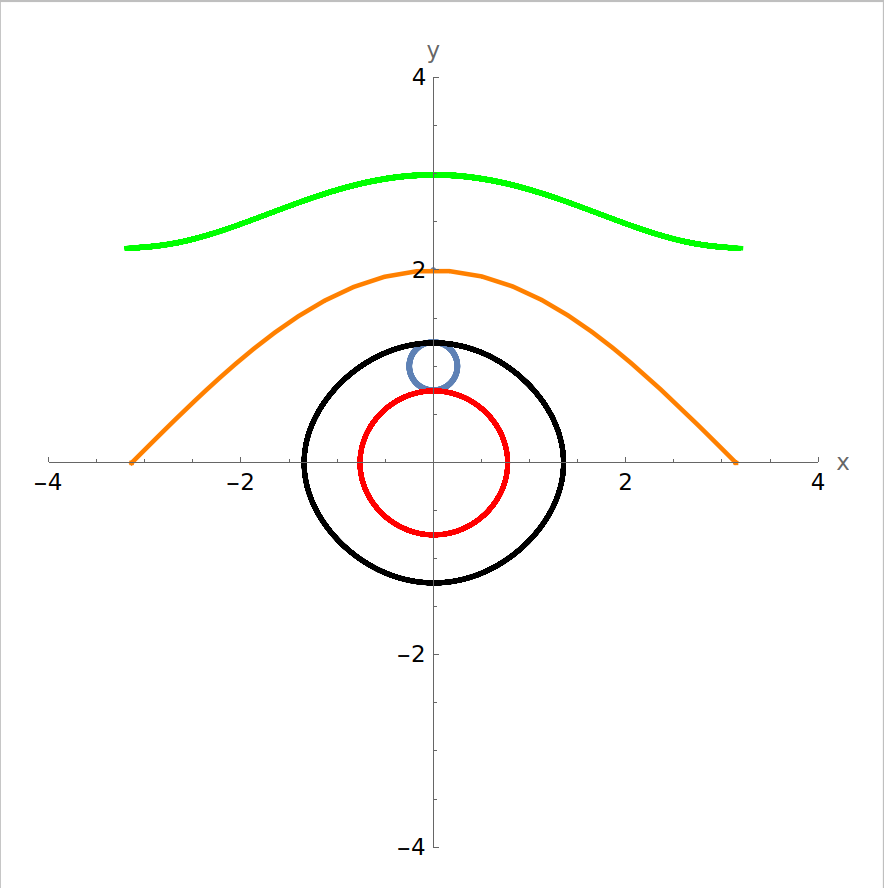
\includegraphics[width=.3\textwidth]{2_nlpendulum1}}
	\subfigure[$t = 26$]{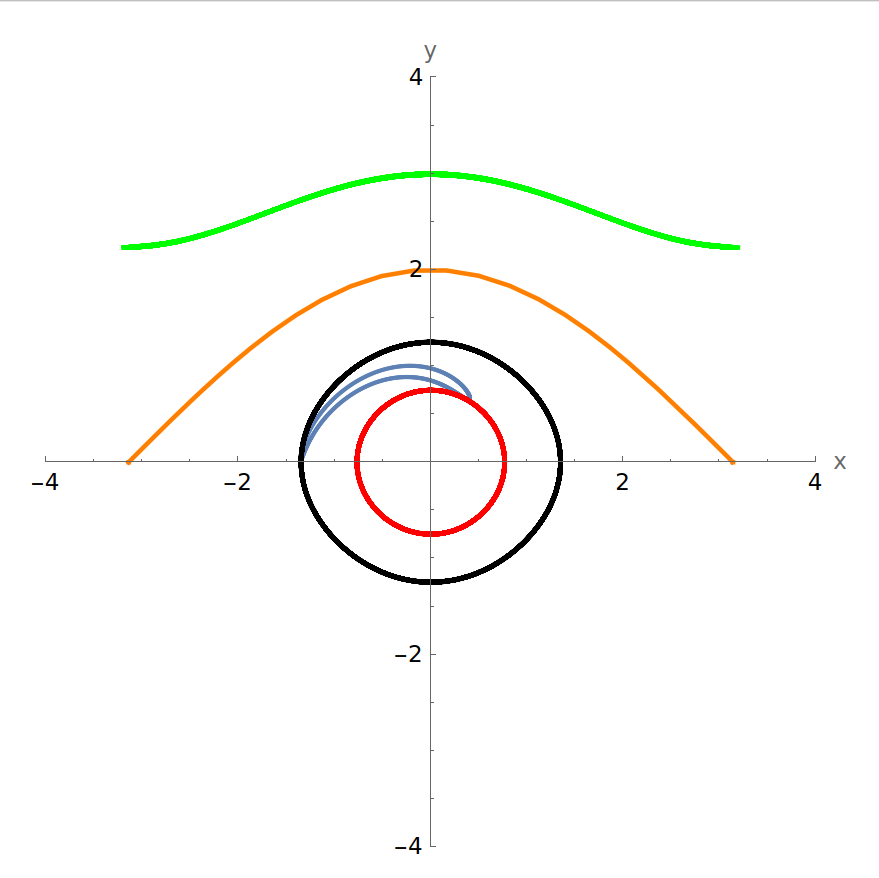
\includegraphics[width=.3\textwidth]{2_nlpendulum2}}
	\subfigure[$t = 50$]{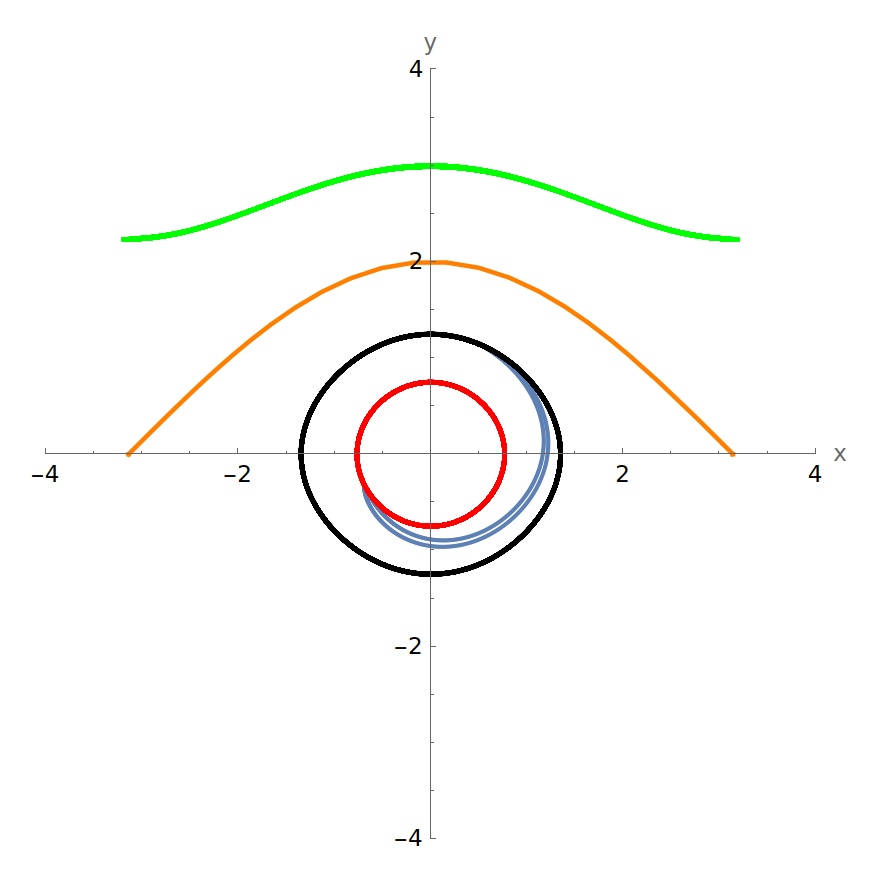
\includegraphics[width=.3\textwidth]{2_nlpendulum}}
	
	\caption{Phase plot for the non-linear pendulum. The inner and outer ellipses bounding ellipses are shown in red and black. The points lying on the boundary of the initial circle and subsequent motion are shown in blue. The seperatrix is shown in orange, and an unbound orbit is shown in green.}
	\label{FIGURE LABEL}
\end{figure}

\end{enumerate}
\end{enumerate}


    \part{Lagrangian Mechanics}
    \chapter{Variational principles}\label{chap3}



    \chapter{Lagrangian mechanics on manifolds}\label{chap4}

    \chapter{Oscillations}\label{chap5}

    \chapter{Rigid Bodies}\label{chap6}

    \part{Hamiltonian Mechanics}
    \chapter{Differential Forms}\label{chap7}

    \chapter{Symplectic manifolds}\label{chap8}

    \chapter{Canonical formalism}\label{chap9}

    \chapter{Introduction to perturbation theory}\label{chap10}

    \renewcommand{\sectionmark}[1]{\markright{#1}}
    \addcontentsline{toc}{chapter}{Bibliography}
    \bibliographystyle{splncs04.bst}
    \bibliography{refs}

    \appendix
    \pretocmd{\chapter}{\pagenumbering{arabic}
	                          \renewcommand*{\thepage}{\thechapter.\arabic{page}}
                           }{}{} 
    \include{appendix1}
\end{document}